% !TEX program = pdflatex
% !TEX options = -synctex=1 -interaction=nonstopmode -file-line-error -shell-escape "%DOC%"

\documentclass[crop,tikz,convert={outext=.svg,command=\unexpanded{pdf2svg \infile\space\outfile}},multi=false]{standalone}

\usetikzlibrary{calc,decorations.pathreplacing,backgrounds}
\usepackage{amsfonts,amssymb,amsthm,amsmath}

\definecolor{mycolor1}{RGB}{27,158,119}
\definecolor{mycolor2}{RGB}{217,95,2}
\definecolor{mycolor3}{RGB}{117,112,179}
\definecolor{mycolor4}{RGB}{231,41,138}


\newcommand{\fitellipsis}[2] % first and second node names without parentheses
{\draw let \p1=(#1), \p2=(#2), \n1={atan2(\y2-\y1,\x2-\x1)}, \n2={veclen(\y2-\y1,\x2-\x1)}
    in ($ (\p1)!0.5!(\p2) $) ellipse [x radius=\n2/2+1cm, y radius=1.5cm, rotate=\n1];
}

\begin{document}
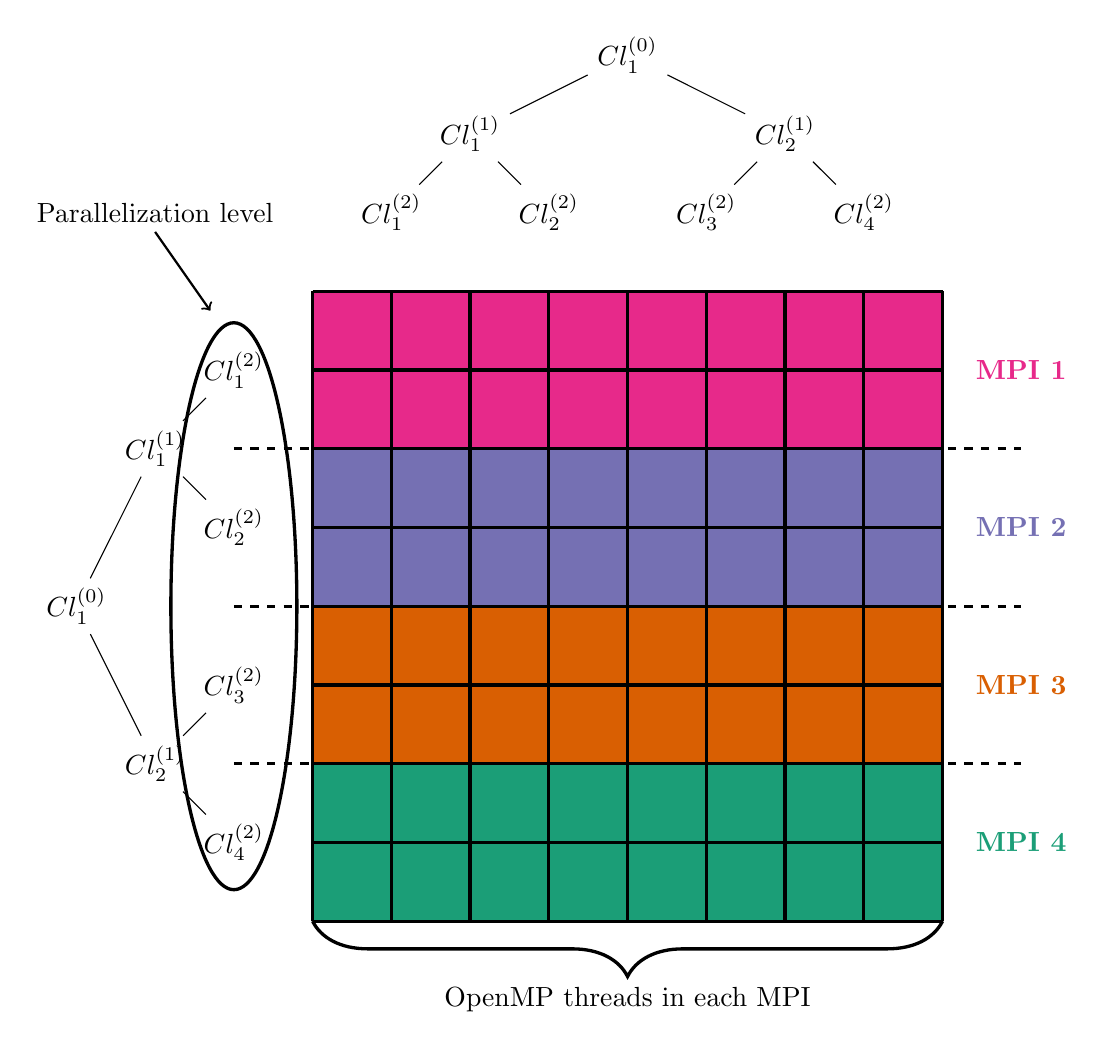
\begin{tikzpicture}

    % Matrix
    \draw[very thick] (0,0) grid (8,8);

    % Source tree
    \node at (4,11) (Is00) {\(Cl^{(0)}_1\)} ;
    \node at (2,10) (Is10) {\(Cl^{(1)}_1\)} ;
    \node at (6,10) (Is11) {\(Cl^{(1)}_2\)} ;
    \node at (1,9) (Is20) {\(Cl^{(2)}_1\)} ;
    \node at (3,9) (Is21) {\(Cl^{(2)}_2\)} ;
    \node at (5,9) (Is22) {\(Cl^{(2)}_3\)} ;
    \node at (7,9) (Is23) {\(Cl^{(2)}_4\)} ;

    \draw (Is00) -- (Is10);
    \draw (Is00) -- (Is11);
    \draw (Is10) -- (Is20);
    \draw (Is10) -- (Is21);
    \draw (Is11) -- (Is22);
    \draw (Is11) -- (Is23);

    % Target tree
    \node at (-3,4) (It00) {\(Cl^{(0)}_1\)} ;
    \node at (-2,2) (It10) {\(Cl^{(1)}_2\)} ;
    \node at (-2,6) (It11) {\(Cl^{(1)}_1\)} ;
    \node at (-1,1) (It20) {\(Cl^{(2)}_4\)} ;
    \node at (-1,3) (It21) {\(Cl^{(2)}_3\)} ;
    \node at (-1,5) (It22) {\(Cl^{(2)}_2\)} ;
    \node at (-1,7) (It23) {\(Cl^{(2)}_1\)} ;

    \draw (It00) -- (It10);
    \draw (It00) -- (It11);
    \draw (It10) -- (It20);
    \draw (It10) -- (It21);
    \draw (It11) -- (It22);
    \draw (It11) -- (It23);

    % Parallelization level
    \draw[very thick] let \p1=(It20), \p2=(It23), \n1={atan2(\y2-\y1,\x2-\x1)}, \n2={veclen(\y2-\y1,\x2-\x1)} in ($ (\p1)!0.5!(\p2) $) ellipse [x radius=\n2/2+0.6cm, y radius=0.80cm, rotate=\n1];
    \node at (-2,9) (Annotation) {Parallelization level};
    \draw [->,thick] (Annotation.south) -- +(0.7,-10mm);

    % Partition
    \draw[very thick,dashed] (-1,2) -- (9,2);
    \draw[very thick,dashed] (-1,4) -- (9,4);
    \draw[very thick,dashed] (-1,6) -- (9,6);
    \node[mycolor1] at (9,1) {\textbf{MPI 4}};
    \node[mycolor2] at (9,3) {\textbf{MPI 3}};
    \node[mycolor3] at (9,5) {\textbf{MPI 2}};
    \node[mycolor4] at (9,7) {\textbf{MPI 1}};

    % OpenMP
    \draw [decorate,decoration={brace,amplitude=20pt},very thick] (8,0) -- (0,0);
    \node at (4,-1) {OpenMP threads in each MPI};
    % \draw [decorate,decoration={brace,amplitude=10pt},xshift=-4pt,yshift=0pt]
    % (0.5,0.5) -- (0.5,5.0) node [black,midway,xshift=-0.6cm] 

    % Blocks
    \begin{scope}[on background layer]
        \fill[mycolor1] (0,0) rectangle (8,2);
        \fill[mycolor2] (0,2) rectangle (8,4);
        \fill[mycolor3] (0,4) rectangle (8,6);
        \fill[mycolor4] (0,6) rectangle (8,8);
    \end{scope}

\end{tikzpicture}
\end{document}
